\documentclass[a4j]{jarticle}
%\documentclass{jarticle}
\usepackage{conf_jst}
\usepackage{graphicx}
\usepackage{multirow}
\usepackage{listings}
\usepackage{plistings}
%\usepackage{fancyheadings}

\oddsidemargin -10mm % 15mm - 1inch(25.4mm)
\evensidemargin -10mm
\textwidth 180mm  % A4幅210mm - 15*2mm
%\topmargin -10.4mm % 25mm - 25.4
\topmargin -10mm % 25mm - 25.4
\textheight 257mm % A4高さ297mm - 25*2mm
%\headheight 10mm
%\headsep 10mm

\setcounter{figure}{0}              %ここで図番号の変更が行えます.
\setcounter{table}{0}               %ここで表番号の変更が行えます.
\setcounter{equation}{0}            %ここで式番号の変更が行えます.

\if0
\def\thefigure{\thesection\arabic{figure}}      %図番号の形式設定
\def\thetable{\thesection\arabic{table}}        %表番号の形式設定
\def\theequation{\thesection\arabic{equation}}  %数式番号の形式設定
\fi

\pagestyle{plain}

\title{2020/03/10 研究報告資料}
\author{氏名:田村 玄}
\date{期間:2019/11/15 ~ 2020/03/22}

\begin{document}
\maketitle

\section{これはセクションテストです}

hoge

\subsection{これはサブセクションテストです}

hoge

\subsubsection{これはサブサブセクションのテストです}

piyo

図の挿入テスト

\begin{figure}
\centering
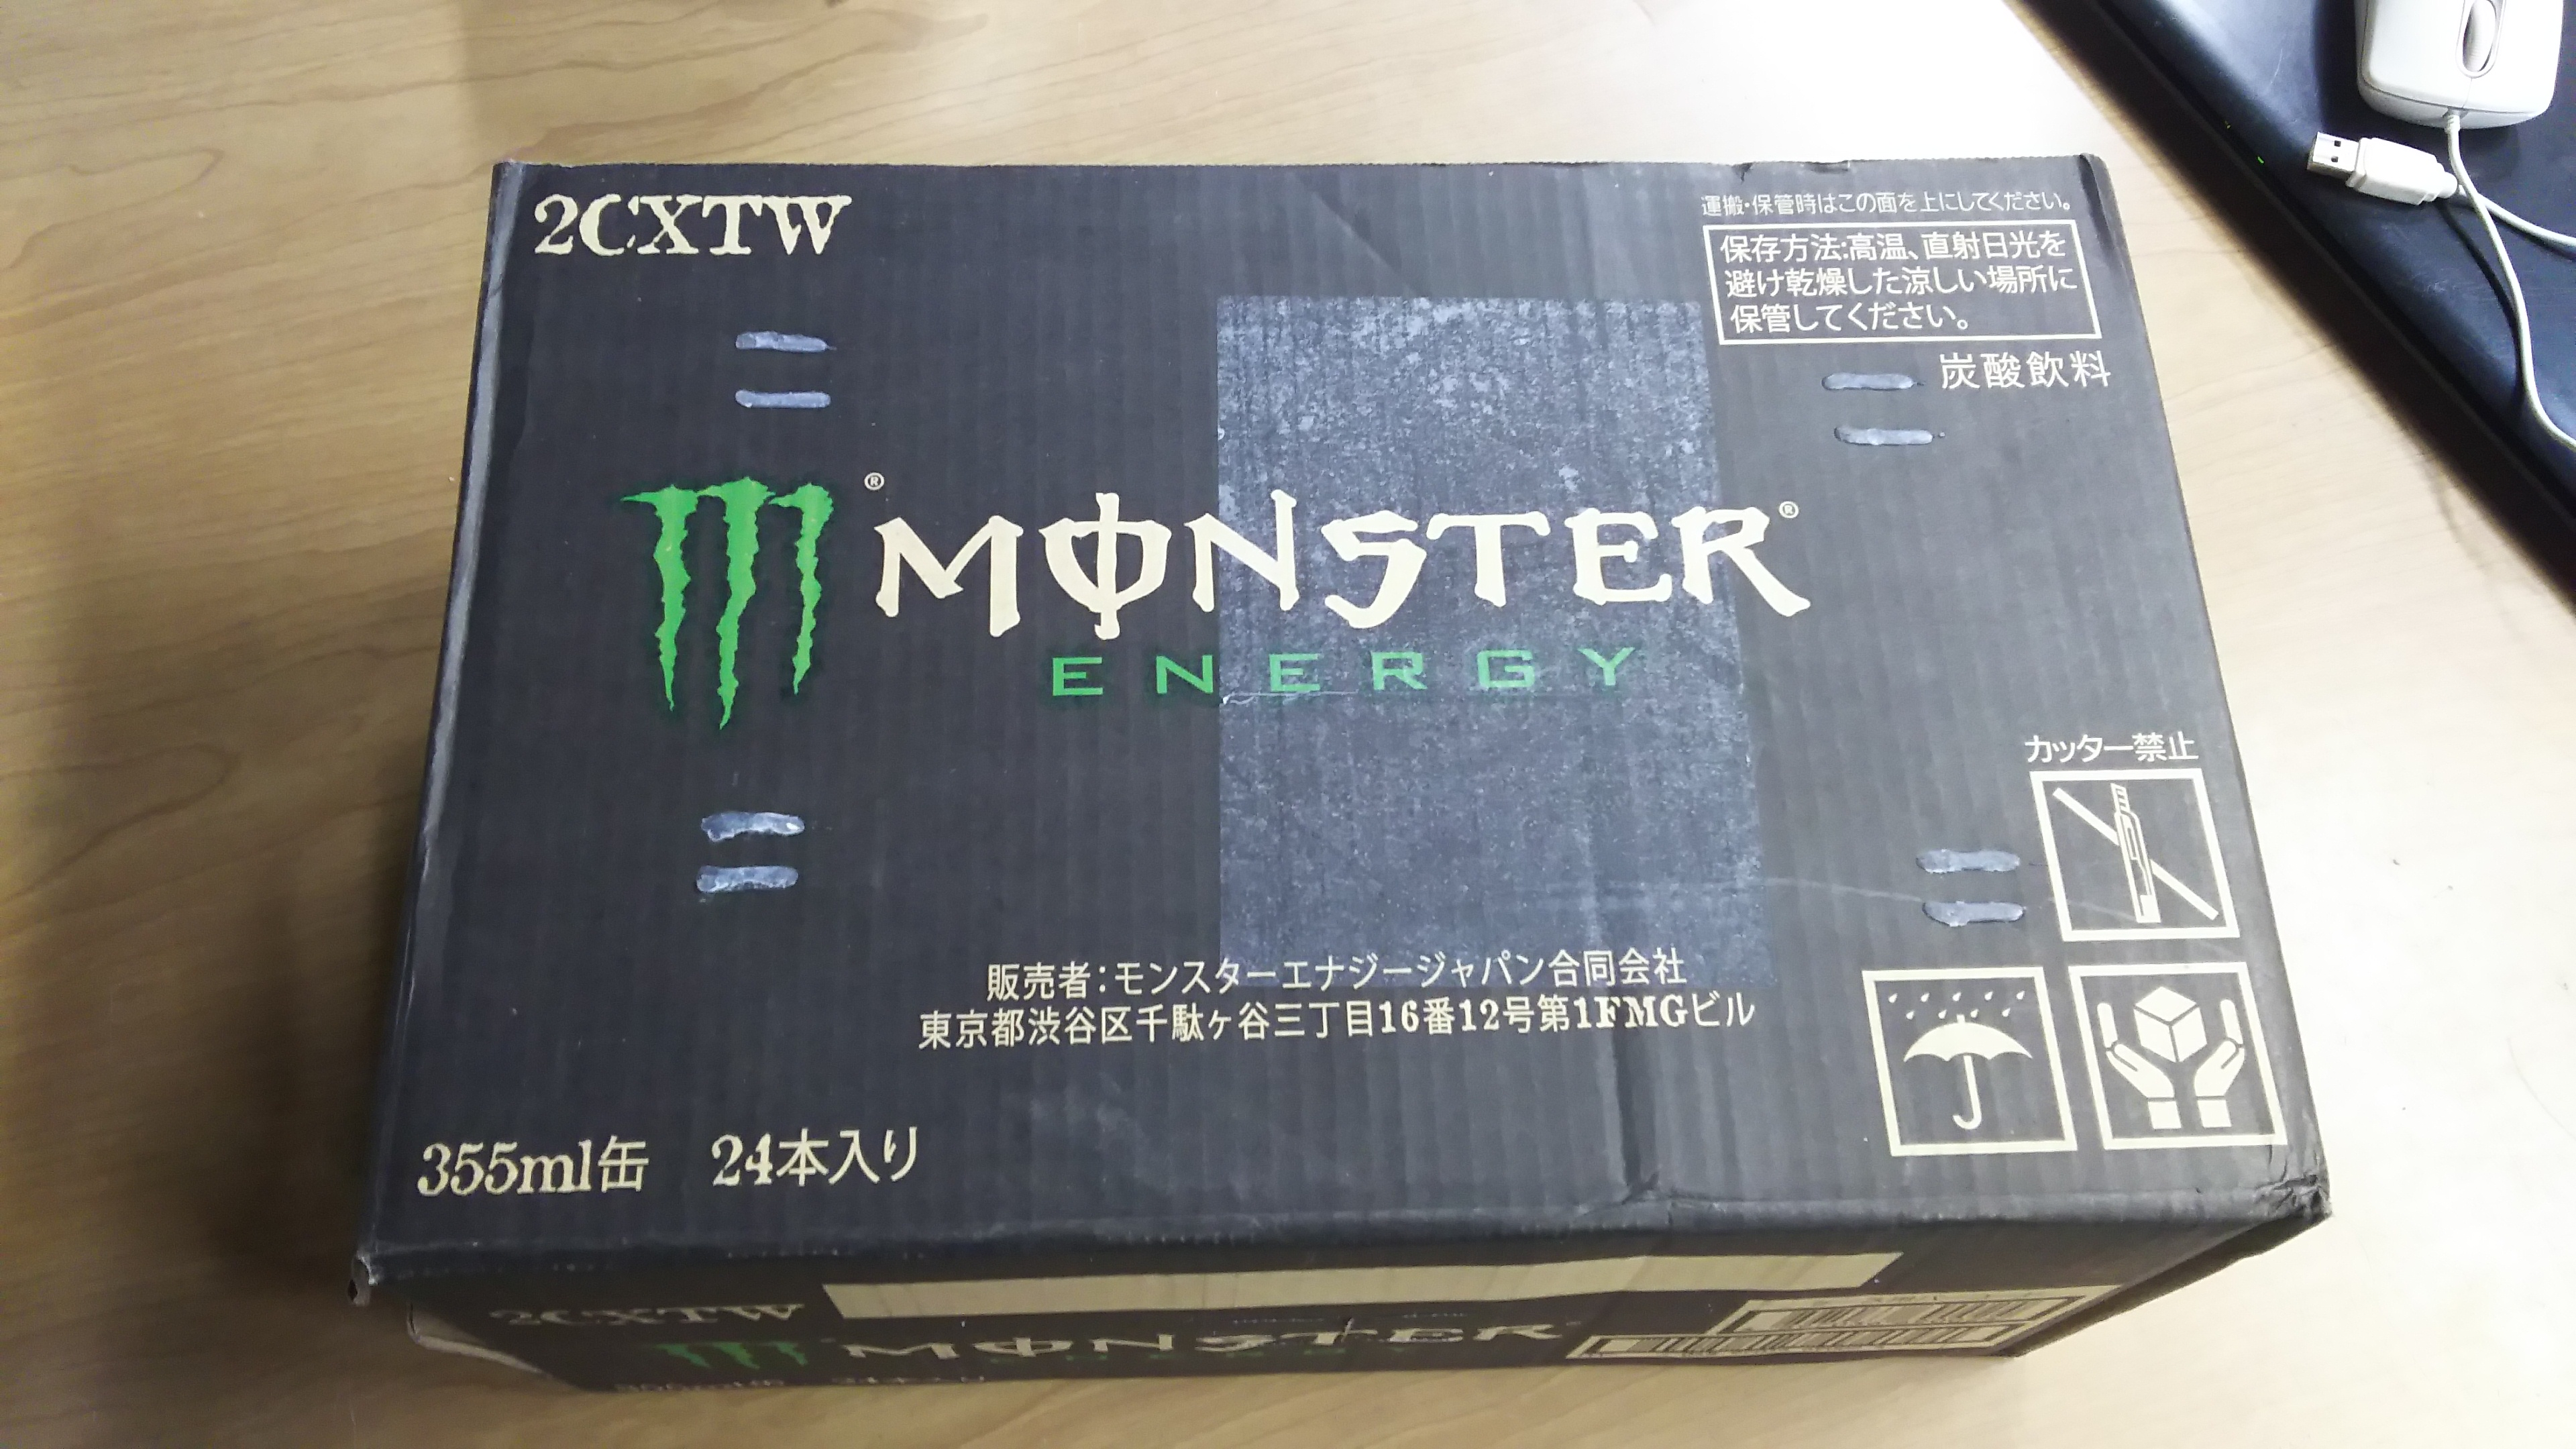
\includegraphics{DSC_0358.eps}
\caption{モンスターエナジー}
\end{figure}

\end{document}
